
\begin{figure}[h]
\centering
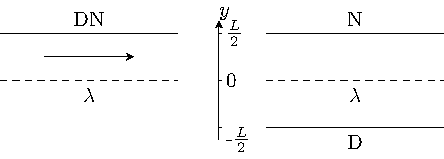
\includegraphics[width=\columnwidth]{fig_gnd_dn_lambda.pdf}
\caption{Partition function of Hamiltonian with DN and $\lambda$ boundary conditions. We unfold the cylinder and the new stripe has N and D boundary conditions on the top and bottom plus a $\lambda$ junction in the middle. The length $L$ here is the height of the unfolded cylinder $2\pi$. }
\label{fig:Fig_gnd_dn_lambda}
\end{figure}

In this appendix, we calculate the amplitude for the setup shown in Fig.~\ref{fig:Fig_gnd_dn_lambda}. In particular, the unfolded configuration has D/N boundary conditions at $y = \pm \frac{L}{2}$ and conformal interface $\lambda$ at $y = 0$. The general solutions can be written as
\begin{equation}
\label{eq:normalized_f}
f(k, y) = 
\left\lbrace
\begin{aligned}
  A_1 e^{i kt} \cos\left(ky +\frac{1}{2}kL \right) &  \quad y < 0  \\
  A_2 e^{ikt}  \sin\left(ky - \frac{1}{2}kL \right) & \quad y > 0 .  \\
\end{aligned} \right. 
\end{equation}
As demonstrated in Sec.~\ref{sec_sub:general_formulation}, if we denote $f(k,y<0)\equiv\phi_1$ and $f(k,y>0)\equiv\phi_2$, the boundary condition at the junction becomes
\begin{eqnarray}\begin{aligned}
\frac{\partial_x \phi_1}{ \partial_t \phi_1} = \lambda^2 \frac{\partial_x \phi_2}{ \partial_t \phi_2} = \tan^2 \theta\frac{\partial_x \phi_2}{ \partial_t \phi_2}, \quad \theta \in \left[0,\frac{\pi}{2} \right]  ,
\end{aligned}\end{eqnarray}
which implies
\begin{equation}
\label{eq:momentum_gnd_dn_lambda}
k = \frac{2\pi}{L}\left( n \pm \frac{\theta}{\pi} \right),  \quad n\in\mathbb{Z}.
\end{equation}
It is evident that the momentum $k$ is shifted from an integer multiple of $\frac{2\pi}{L}$ due to the $\lambda$ boundary condition in the middle. 

The normalized eigenfunctions in Eq.~\eqref{eq:normalized_f} serves as an orthonormal basis in the mode expansion, we thus have
\begin{equation}
\label{eq:H_in_gnd_dn_lambda}
H = \frac{1}{2} \sum_{n \in \mathbb{Z} } |k|  \left(a^{\dagger}_n a_n + \frac{1}{2} \right) ,
\end{equation}
where the momentum $k$ is defined in Eq.~\eqref{eq:momentum_gnd_dn_lambda}, and the creation and annihilation operators are defined as usual
\begin{equation}
\begin{aligned}
a_n = \frac{1}{\sqrt{2}} \left( \sqrt{ |k|g} \phi_n + \frac{i }{\sqrt{|k|g} }\pi_n  \right) ,\\
a^{\dagger}_n = \frac{1}{\sqrt{2}} \left( \sqrt{ |k|g} \phi_n - \frac{i }{\sqrt{|k|g} }\pi_n  \right) .\\
\end{aligned}
\end{equation}

The Casimir energy is the vacuum energy brought up by the finite size of the setup. From Eq.~\eqref{eq:H_in_gnd_dn_lambda} and using $x\equiv \frac{\theta}{\pi}$ in Eq.~\eqref{eq:momentum_gnd_dn_lambda}, we have
\begin{equation}
\begin{aligned}
E_c &= \frac{1}{4} \sum_{n \in \mathbb{Z}} | k| = \frac{\pi}{2L} \left( \sum_{n \in \mathbb{Z}}  | n + x | + \sum_{n \in \mathbb{Z}}  | n - x |  \right) \\
&= \frac{\pi}{2L} \Bigg( \sum_{n\ge 0 }  ( n + x ) + \sum_{n< 0 }  ( -n - x )  \\
&\quad \quad + \sum_{n \le 0}  (- n + x ) + \sum_{n > 0} ( n- x )  \Bigg) \\
&= \frac{\pi}{2L} \left( 2\sum_{n\ge 0 }  ( n + x ) + 2\sum_{n > 0} ( n- x )  \right).
\end{aligned}
\end{equation}
We use the Hurwitz zeta function
\begin{equation}
\zeta_{\rm H}(s,x) = \sum_{n=0}^\infty\frac{1}{(n+x)^s}
\end{equation}
to regularize the sum, 
\begin{equation}
\begin{aligned}
E_c &= \frac{\pi}{L} \Big[\sum_{n \ge 0 } ( n + x )^{-s} + \sum_{n \ge 0 }  ( n - x)^{-s}  -  (-x)^{-s} \Big]\Big|_{s = -1} \\
&= \frac{\pi}{L} \left[ \zeta_{\rm H}( -1, x ) + \zeta_{\rm H}( -1, -x ) +  x \right] \\
&= \frac{1}{2} \left( - x^2 + x - \frac{1}{6}\right),
\end{aligned}
\end{equation}
where in the last line we use $L = 2\pi$ for the unfolded geometry. 

Thus the free energy in the large $\beta$ limit is
\begin{equation}
F = \beta E_c = - \frac{\beta}{2} B_2( x) ,
\end{equation}
which agrees with the boundary state calculation in Sec.~\ref{app:lambda_12}. 

%%% Local Variables:
%%% TeX-master: "bCFT_paper"
%%% TeX-PDF-mode: t
%%% End:
